\documentclass[]{book}
\usepackage{lmodern}
\usepackage{amssymb,amsmath}
\usepackage{ifxetex,ifluatex}
\usepackage{fixltx2e} % provides \textsubscript
\ifnum 0\ifxetex 1\fi\ifluatex 1\fi=0 % if pdftex
  \usepackage[T1]{fontenc}
  \usepackage[utf8]{inputenc}
\else % if luatex or xelatex
  \ifxetex
    \usepackage{mathspec}
  \else
    \usepackage{fontspec}
  \fi
  \defaultfontfeatures{Ligatures=TeX,Scale=MatchLowercase}
\fi
% use upquote if available, for straight quotes in verbatim environments
\IfFileExists{upquote.sty}{\usepackage{upquote}}{}
% use microtype if available
\IfFileExists{microtype.sty}{%
\usepackage{microtype}
\UseMicrotypeSet[protrusion]{basicmath} % disable protrusion for tt fonts
}{}
\usepackage[margin=1in]{geometry}
\usepackage{hyperref}
\hypersetup{unicode=true,
            pdftitle={A Tidy Introduction To Statistical Learning},
            pdfauthor={Beau Lucas},
            pdfborder={0 0 0},
            breaklinks=true}
\urlstyle{same}  % don't use monospace font for urls
\usepackage{natbib}
\bibliographystyle{apalike}
\usepackage{color}
\usepackage{fancyvrb}
\newcommand{\VerbBar}{|}
\newcommand{\VERB}{\Verb[commandchars=\\\{\}]}
\DefineVerbatimEnvironment{Highlighting}{Verbatim}{commandchars=\\\{\}}
% Add ',fontsize=\small' for more characters per line
\usepackage{framed}
\definecolor{shadecolor}{RGB}{248,248,248}
\newenvironment{Shaded}{\begin{snugshade}}{\end{snugshade}}
\newcommand{\KeywordTok}[1]{\textcolor[rgb]{0.13,0.29,0.53}{\textbf{#1}}}
\newcommand{\DataTypeTok}[1]{\textcolor[rgb]{0.13,0.29,0.53}{#1}}
\newcommand{\DecValTok}[1]{\textcolor[rgb]{0.00,0.00,0.81}{#1}}
\newcommand{\BaseNTok}[1]{\textcolor[rgb]{0.00,0.00,0.81}{#1}}
\newcommand{\FloatTok}[1]{\textcolor[rgb]{0.00,0.00,0.81}{#1}}
\newcommand{\ConstantTok}[1]{\textcolor[rgb]{0.00,0.00,0.00}{#1}}
\newcommand{\CharTok}[1]{\textcolor[rgb]{0.31,0.60,0.02}{#1}}
\newcommand{\SpecialCharTok}[1]{\textcolor[rgb]{0.00,0.00,0.00}{#1}}
\newcommand{\StringTok}[1]{\textcolor[rgb]{0.31,0.60,0.02}{#1}}
\newcommand{\VerbatimStringTok}[1]{\textcolor[rgb]{0.31,0.60,0.02}{#1}}
\newcommand{\SpecialStringTok}[1]{\textcolor[rgb]{0.31,0.60,0.02}{#1}}
\newcommand{\ImportTok}[1]{#1}
\newcommand{\CommentTok}[1]{\textcolor[rgb]{0.56,0.35,0.01}{\textit{#1}}}
\newcommand{\DocumentationTok}[1]{\textcolor[rgb]{0.56,0.35,0.01}{\textbf{\textit{#1}}}}
\newcommand{\AnnotationTok}[1]{\textcolor[rgb]{0.56,0.35,0.01}{\textbf{\textit{#1}}}}
\newcommand{\CommentVarTok}[1]{\textcolor[rgb]{0.56,0.35,0.01}{\textbf{\textit{#1}}}}
\newcommand{\OtherTok}[1]{\textcolor[rgb]{0.56,0.35,0.01}{#1}}
\newcommand{\FunctionTok}[1]{\textcolor[rgb]{0.00,0.00,0.00}{#1}}
\newcommand{\VariableTok}[1]{\textcolor[rgb]{0.00,0.00,0.00}{#1}}
\newcommand{\ControlFlowTok}[1]{\textcolor[rgb]{0.13,0.29,0.53}{\textbf{#1}}}
\newcommand{\OperatorTok}[1]{\textcolor[rgb]{0.81,0.36,0.00}{\textbf{#1}}}
\newcommand{\BuiltInTok}[1]{#1}
\newcommand{\ExtensionTok}[1]{#1}
\newcommand{\PreprocessorTok}[1]{\textcolor[rgb]{0.56,0.35,0.01}{\textit{#1}}}
\newcommand{\AttributeTok}[1]{\textcolor[rgb]{0.77,0.63,0.00}{#1}}
\newcommand{\RegionMarkerTok}[1]{#1}
\newcommand{\InformationTok}[1]{\textcolor[rgb]{0.56,0.35,0.01}{\textbf{\textit{#1}}}}
\newcommand{\WarningTok}[1]{\textcolor[rgb]{0.56,0.35,0.01}{\textbf{\textit{#1}}}}
\newcommand{\AlertTok}[1]{\textcolor[rgb]{0.94,0.16,0.16}{#1}}
\newcommand{\ErrorTok}[1]{\textcolor[rgb]{0.64,0.00,0.00}{\textbf{#1}}}
\newcommand{\NormalTok}[1]{#1}
\usepackage{longtable,booktabs}
\usepackage{graphicx,grffile}
\makeatletter
\def\maxwidth{\ifdim\Gin@nat@width>\linewidth\linewidth\else\Gin@nat@width\fi}
\def\maxheight{\ifdim\Gin@nat@height>\textheight\textheight\else\Gin@nat@height\fi}
\makeatother
% Scale images if necessary, so that they will not overflow the page
% margins by default, and it is still possible to overwrite the defaults
% using explicit options in \includegraphics[width, height, ...]{}
\setkeys{Gin}{width=\maxwidth,height=\maxheight,keepaspectratio}
\IfFileExists{parskip.sty}{%
\usepackage{parskip}
}{% else
\setlength{\parindent}{0pt}
\setlength{\parskip}{6pt plus 2pt minus 1pt}
}
\setlength{\emergencystretch}{3em}  % prevent overfull lines
\providecommand{\tightlist}{%
  \setlength{\itemsep}{0pt}\setlength{\parskip}{0pt}}
\setcounter{secnumdepth}{5}
% Redefines (sub)paragraphs to behave more like sections
\ifx\paragraph\undefined\else
\let\oldparagraph\paragraph
\renewcommand{\paragraph}[1]{\oldparagraph{#1}\mbox{}}
\fi
\ifx\subparagraph\undefined\else
\let\oldsubparagraph\subparagraph
\renewcommand{\subparagraph}[1]{\oldsubparagraph{#1}\mbox{}}
\fi

%%% Use protect on footnotes to avoid problems with footnotes in titles
\let\rmarkdownfootnote\footnote%
\def\footnote{\protect\rmarkdownfootnote}

%%% Change title format to be more compact
\usepackage{titling}

% Create subtitle command for use in maketitle
\newcommand{\subtitle}[1]{
  \posttitle{
    \begin{center}\large#1\end{center}
    }
}

\setlength{\droptitle}{-2em}
  \title{A Tidy Introduction To Statistical Learning}
  \pretitle{\vspace{\droptitle}\centering\huge}
  \posttitle{\par}
  \author{Beau Lucas}
  \preauthor{\centering\large\emph}
  \postauthor{\par}
  \predate{\centering\large\emph}
  \postdate{\par}
  \date{2018-04-27}

\usepackage{booktabs}
\usepackage{amsthm}
\makeatletter
\def\thm@space@setup{%
  \thm@preskip=8pt plus 2pt minus 4pt
  \thm@postskip=\thm@preskip
}
\makeatother

\usepackage{amsthm}
\newtheorem{theorem}{Theorem}[chapter]
\newtheorem{lemma}{Lemma}[chapter]
\theoremstyle{definition}
\newtheorem{definition}{Definition}[chapter]
\newtheorem{corollary}{Corollary}[chapter]
\newtheorem{proposition}{Proposition}[chapter]
\theoremstyle{definition}
\newtheorem{example}{Example}[chapter]
\theoremstyle{definition}
\newtheorem{exercise}{Exercise}[chapter]
\theoremstyle{remark}
\newtheorem*{remark}{Remark}
\newtheorem*{solution}{Solution}
\begin{document}
\maketitle

{
\setcounter{tocdepth}{1}
\tableofcontents
}
\chapter*{Preface}\label{preface}
\addcontentsline{toc}{chapter}{Preface}

This book will serve as a source of notes and exercise solutions for
\emph{An Introduction to Statistical Learning}. My approach will be
centered around the \texttt{tidyverse}. This is not a replacement for
the book, which should be read front to back by all machine learning
enthusiasts.

Chapter names will line up, and certain subheadings will also match.
Sometimes my notes will contain text lifted straight from the book
without modification. This is not an attempt to plagiarize or claim
their writing as my own. My goal is for this bookdown project to be a
quick stop for machine learning enthusiasts to reference high-level
ideas from ISLR in a modern media format.

\chapter{Introduction}\label{intro}

\begin{center}\rule{0.5\linewidth}{\linethickness}\end{center}

\section{An Overview of Statistical
Learning}\label{an-overview-of-statistical-learning}

Statistical learning is focused on supervised and unsupervised modeling
and prediction.

\section{Data Sets Used in Labs and
Exercises}\label{data-sets-used-in-labs-and-exercises}

All data sets used in this book can be found in \texttt{ISLR} and
\texttt{MASS} packages, with some also being found in the base
\texttt{R} distribution.

We will utilize the \texttt{tidyverse} ecosystem to tackle the exercises
and labs, as the \texttt{R} code found in the original textbook is
outdated.

\begin{Shaded}
\begin{Highlighting}[]
\KeywordTok{require}\NormalTok{(ISLR)}
\KeywordTok{require}\NormalTok{(MASS)}
\KeywordTok{require}\NormalTok{(tidyverse)}
\end{Highlighting}
\end{Shaded}

\section{Book Website}\label{book-website}

The website and free PDF for the book can be found here:

\href{http://www-bcf.usc.edu/~gareth/ISL/}{www.statlearning.com}
\href{https://www.youtube.com/channel/UC4OWDcPB1peiBXDfCSZ3h-w}{Youtube
- Statistical Learning}

\chapter{Statistical Learning}\label{statistical-learning}

\begin{center}\rule{0.5\linewidth}{\linethickness}\end{center}

\section{What is Statistical
Learning?}\label{what-is-statistical-learning}

Methods to estimate functions that connect inputs to outputs.

If there exists a quantitative response variable \(Y\) and \(p\)
different predictors (\(X_1\), \(X_2\), \ldots{}, \(X_p\)), we can write
this relationship as:

\(Y = f(X) + ε\)

\subsection{\texorpdfstring{Why Estimate
\emph{\(f\)}?}{Why Estimate f?}}\label{why-estimate-f}

\subsubsection{Prediction}\label{prediction}

We can predict Y using:

\(\hat{Y} = \hat{f}(X)\)

Accuracy of \(Y\) is dependant on:

\begin{itemize}
\tightlist
\item
  \emph{reducible error}

  \begin{itemize}
  \tightlist
  \item
    \(\hat{f}\) will never be perfect estimate of \(f\), and model can
    always be potentially improved
  \item
    Even if \(\hat{f} = f\), prediction would still have some error
  \end{itemize}
\item
  \emph{irreducible error}

  \begin{itemize}
  \tightlist
  \item
    Because \(Y\) is also a function of random \(ε\), there will alwayas
    be variability
  \item
    We cannot reduce the error introduced by \(ε\)
  \end{itemize}
\end{itemize}

\subsubsection{Inference}\label{inference}

How does \(Y\) respond to changes in \(X_1, X_2, ..., X_p\)?

\subsection{\texorpdfstring{How do we estimate
\emph{\(f\)}?}{How do we estimate f?}}\label{how-do-we-estimate-f}

\begin{itemize}
\tightlist
\item
  Use \emph{training data} to train method
\item
  \(x_ij\) is value of \(j\)th predictor for observation \(i\), \(y_i\)
  is value of response variable

  \begin{itemize}
  \tightlist
  \item
    \(i = 1, 2, ..., n\), \(j = 1, 2, ..., p\)
  \end{itemize}
\item
  Using training data, apply statistical learning method estimate
  unknown function \(f\)
\item
  Most statistical learning methods can be characterized as either
  \emph{parametric} or \emph{non-parametric}
\end{itemize}

\subsubsection{Parametric Methods}\label{parametric-methods}

Two-step model-based approach:

\begin{enumerate}
\def\labelenumi{\arabic{enumi}.}
\tightlist
\item
  Make an assumption about functional form of \(f\), such as ``\(f\) is
  linear in \(X\)''
\item
  Perform procedure that uses training data to train the model

  \begin{itemize}
  \tightlist
  \item
    In case of linear model, this procedure estimates parameters
    \(β_0, β_1, ..., β_p\)
  \item
    Most common approach to fit linear model is \emph{(ordinary) least
    squares}
  \end{itemize}
\end{enumerate}

This is \emph{parametric}, as it reduces the problem of estimating \(f\)
down to one of estimating a set of parameters. Problems that can arise:

\begin{itemize}
\tightlist
\item
  Model will not match the true unknown form of \(f\)
\item
  If model is made more \emph{flexible}, which generally requires
  estimating a greater number of parameters, \emph{overfitting} can
  occur
\end{itemize}

\subsubsection{Non-parametric Methods}\label{non-parametric-methods}

Non-parametric methods do not make assumptions about the form of \(f\).
An advantage of this is that they have the potential to fit a wider
range of possible shapes for \(f\). A disadvantage is that, because
there are no assumptions about the form of \(f\), the problem of
estimating \(f\) is not reduced to a set number of parameters. This
means more observations are needed compared to a parametric approach to
estimate \(f\) accurately.

\subsection{The Trade-Off Between Prediction Accuracy and Model
Interpretability}\label{the-trade-off-between-prediction-accuracy-and-model-interpretability}

Restrictive models are much more intepretable than flexible ones.
Flexible approaches can be so complicated that it is hard to understand
how predictors affect the response.

If inference is the goal, simple and inflexible methods are easier to
interpret. For prediction, accuracy is the biggest concern. However,
flexible models are more prone to overfitting.

\subsection{Supervised Versus Unsupervised
Learning}\label{supervised-versus-unsupervised-learning}

Most machine learning methods can be split into \emph{supervised} or
\emph{unsupervised} categories. Most of this textbook involves
supervised learning methods, in which a model that captures the
relationship between predictors and response measurements is fitted. The
goal is to accurately predict the response variables for future
observations, or to understand the relationship between the predictors
and response.

Unsupervised learning takes place when we have a set of observations and
a vector of measurements \(x_i\), but no response \(y_i\). We can
examine the relationship between the variables or between the
observations. A popular method of unsupervised learning is
\href{https://en.wikipedia.org/wiki/Cluster_analysis}{cluster analysis},
in which observations are grouped into distinct groups based on their
vector of measurements \(x_i\). An example of this would be a company
segmenting survey respondents based on demographic data, in which the
goal is to ascertain some idea about potential spending habits without
possessing this data.

Clustering has some drawbacks. It works best when the groups are
significantly distinct from each other. In reality, it is rare for data
to exhibit this characteristic. There is often overlap between
observations in different groups, and clustering will inevitably place a
number of observations in the wrong groups. Further more, visualization
of clusters breaks down as the dimensionality of data increases. Most
data contains at least several, if not dozens, of variables.

It is not always clear-cut whether a problem should be handled with
supervised or unsupervised learning. There are some scenarios where only
a subset of the observations have response measurements. This is a
\emph{semi-supervised learning} problem, in which a statistical learning
method that can utilize all observations is needed.

\subsection{Regression Versus Classification
Problems}\label{regression-versus-classification-problems}

Variables can be categorized as either \emph{quantitative} or
\emph{qualitative}. Both qualitative and quantatitive predictors can be
used to predict both types of response variables. The more important
part of choosing an appropriate statistical learning method is the type
of the response variable.

\begin{center}\rule{0.5\linewidth}{\linethickness}\end{center}

\section{Assessing Model Accuracy}\label{assessing-model-accuracy}

Every data set is different and there is no one statistical learning
method that works best for all data sets. It is important for any given
data set to find the statistical learning method that produces the best
results. This section presents some concepts that are part of that
decision-making process.

\subsection{Measuring the Quality of
Fit}\label{measuring-the-quality-of-fit}

We need to be able to quantify how well a model's predictions match the
observed data. How close are the model's predicted response values to
the true response values?

In regression,
\href{https://en.wikipedia.org/wiki/Mean_squared_error}{\emph{mean
squared error (MSE)}} is the most commonly-used measure. A small MSE
indicates the predicted responses are very close to the true ones. MSE
used on training data is more accurately referred to as the
\emph{training MSE}.

We are most concerned with the accuracy of the predictions when we apply
our methods to \textbf{previously unseen data}. If you are trying to
predict the value of a stock, your concern is how it performs in the
future, not on known data from the past. Thus, the goal is then
minimizing the \emph{test MSE}, which measures the accuracy of a model
on \textbf{observations that were not used to train the model}. Imagine
a set of observations \((x_0, y_0)\) that were not used to train the
statistical learning method.

\(Ave(y_0 - \hat{f}(x_0))2\)

The goal is to select the model that minimizes the test MSE shown above.
How can we do this?

Sometimes, there is an available test data set full of observations that
were not used in training the model. The test MSE can be evaluated on
these observations, and the learning method which produces the smallest
TSE will be chosen. If no test observations are available, picking the
method that minimizes the training MSE might seem to be a good idea.
However, there is no guarantee that a model with the lowest training MSE
also has the lowest test MSE. Models often work in minimizing the
training MSE, and can end up with large test MSE.

There is a tradeoff in model flexibility, training MSE, and test MSE. A
model that is too flexible can closely match the training data, but
perform poorly on the test data. There is a sweet spot to find between
model flexibility, training MSE, and test MSE that varies for each
unique data set.

\emph{Degrees of freedom} is a quantity that summarizes the flexibility
of a curve, discused more fully in Chapter 7. The more inflexible a
model is, the fewer degrees of freedom.

As model flexibility increases, training MSE will inevitably decrease,
but test MSE may plateau or even rise. A model with a small training MSE
and large test MSE is \emph{overfitting the data}, picking up patterns
on the training data that don't exist in the test data. Since we expect
the training MSE to almost always be lower than the test MSE,
overfitting is a specific case when there exists a less flexible model
with a smaller test MSE.

\subsection{The Bias-Variance
Trade-Off}\label{the-bias-variance-trade-off}

The expected test MSE can be broken down into the sum of three
quantities:

\begin{enumerate}
\def\labelenumi{\arabic{enumi}.}
\tightlist
\item
  the \emph{variance} of \(\hat{f}(x_0)\)
\item
  the squared \emph{bias} of \(\hat{f}(x_0)\)
\item
  the variance of the error terms ε
\end{enumerate}

\(E(y_0 - \hat{f}(x_0)^2 = Var(\hat{f}(x_0)) + [Bias(\hat{f}(x_0))]^2+Var(ε)\)

The formula above defines the \emph{expected test MSE}, which can be
thought of the average test MSE that would be obtained if we repeatedly
estimated \(f\) and tested each at \(x_0\). To minimize expected test
MSE, we need to choose a statistical learning method that achieves both
low variance and low bias. Since variance and squared bias are
nonnegative, the expected test MSE can never be lower than \(Var(ε)\),
the irreducible error.

\emph{Variance} refers to how much \(\hat{f}\) would change if
repeatedly estimated with different training data sets. Methods with
high variance can produce large changes in \(\hat{f}\) through small
changes in the training data. Generally, the more flexible a model it
is, the higher the variance. Following the observations so closely can
cause changes in just a single observation of the training data to
result in significant changes to \(\hat{f}\). More inflexible models,
such as linear regression, are less susceptible to the effects of
changing a single observation.

\emph{Bias} is the error introduced from approximating a complicated
problem by a much simpler model. Fitting a linear regression to data
that is not linear will always lead to high bias, no matter how many
observations are in the training set. More flexible models tend to
result in less bias.

More flexible methods lead to higher variance and lower bias. The rate
of change between the quantities determines at which point the test MSE
is minimized. Bias tends to decrease at a faster rate in the beginning,
causing the test MSE to decline. However, when flexibility reaches a
certain point, variance will begin to increase faster than bias is
decreasing, causing test MSE to rise.

This relationship between bias, variance, and test MSE is known as the
\emph{bias-variance tradeoff}. Here is a good article on it:
\href{http://scott.fortmann-roe.com/docs/BiasVariance.html}{Understanding
the Bias-Variance Tradeoff}

In real-life scenarios where \(f\) is unknown, we cannot explicitly
compute the test MSE, bias, or variance. However, there are methods to
estimate this, such as \emph{cross-validation}, which will be discussed
in Chapter 5.

\subsection{The Classification
Setting}\label{the-classification-setting}

For classification problems where \(y_i,...,y_n\) are qualitative, we
can quantify the accuracy of our estimate by using the \emph{training
error rate}, the proportion of mistakes that are made when applying our
model \(\hat{f}\) to the training observations.

\(1/n\sum_{i=1}^nI(y_i \neq \hat{y_i})\)

\emph{training error rate}

Breaking the formula above down.

\begin{itemize}
\tightlist
\item
  \(\hat{y}_i\) is the predicted class label for the \(i\)th observation
  using \(\hat{f}\)
\item
  \(I(y_i \neq \hat{y_i})\) is an \emph{indicator variable} that equals
  1 if \(y_i \neq \hat{y_i}\), and 0 if \(y_i = \hat{y_i}\)
\item
  If \(I(y_i \neq \hat{y_i})\) = 0, then the \(i\)th observation was
  classified correctly
\end{itemize}

Similar to our regression problems, we are more interested in the
model's performance on test observations not used in training. The
formula below gives us the \emph{test error rate} for a set of
observations of the form \((x_0, y_0)\).

\(Ave(I(y_0 \neq \hat{y_0}))\)

\emph{test error rate}

A good classifier will minimize the above.

\subsubsection{The Bayes Classifier}\label{the-bayes-classifier}

The \emph{test error rate} is minimized by the classifier that assigns
each observation to the most likely class, given its predictor values.
Our decision is then based on finding the value at which the formula
below is largest.

\(Pr(Y = j|X = x_0)\)

If the response values are binomial (let's call them A and B) the
classifier simplifies to:

\(Pr(Y = A|X = x_0) > 0.5\:then\:A,\:else\:B\)

The \emph{Bayes decision boundary} is the point where the probabilities
are equal for both groups. Points on either side of this line are
assigned to the group predicted by the classifier. The \emph{Bayes error
rate} averaged over all possible values of \(X\) is below.

\(1-E(max_jPr(Y = j|X))\)

\emph{Bayes error rate}

The \emph{Bayes error rate} is often greater than zero, as observations
between classes overlap in real-world data.

\subsubsection{K-Nearest Neighbors}\label{k-nearest-neighbors}

Since the true conditional distribution of \(Y\) given \(X\) cannot be
known in real data, the Bayes classifier is used as a ``gold standard''
to compare other models to. Many methods attempt to estimate this
conditional distribution, and then classify an observation based on the
estimated probability. A common method is \emph{K-nearest neighbors
(KNN)}. Given a positive integer \(K\) and a test observation \(x_0\),
KNN then does the following:

\begin{enumerate}
\def\labelenumi{\arabic{enumi}.}
\tightlist
\item
  identifies the \(K\) points in the training data that are closest to
  \(x_0\), represented by \(N_0\)
\item
  estimates conditional probability for class \(j\) as the fraction of
  the points in \(N_0\) whose response values equal \(j\):
\end{enumerate}

\(Pr(Y = j| X = x_0) = 1/K\sum_{i\in N_0}I(y_i = j)\)

\begin{enumerate}
\def\labelenumi{\arabic{enumi}.}
\setcounter{enumi}{2}
\tightlist
\item
  applies Bayes rule and classifies test observation \(x_0\) to class
  with largest probability
\end{enumerate}

KNN can be surprisingly robust to the optimal Bayes classifier. The
choice in \(K\) makes a huge difference. For example, a \(K\) = 1 is
highly flexible, classifying observations based off of the closest
nearby training observation. \(K\) = 100 would do the opposite, basing
its classification off a large pool of training observations compared to
the \(K\) = 1 version. The higher \(K\) value produces a more linear
model. The trade-off between flexibility, training error rate, and test
error rate applies to both classification and regression problems.

\section{Lab: Introduction to R}\label{lab-introduction-to-r}

Finally we get to some \texttt{R} code. This chapter of ISLR introduces
basic \texttt{R} syntax, and most of it is unchanged in my version. This
should all be familiar to anyone who has used R before.

We are going to be working with \texttt{tibbles} as our primary data
structure throughout this book. Please read here:
\href{http://r4ds.had.co.nz/tibbles.html}{tibbles}

\subsubsection{Basic Commands}\label{basic-commands}

Skipping this.

\subsubsection{Graphics (Plotting)}\label{graphics-plotting}

Here we begin to explore the ``tidy'' approach to R. We will abstain
from base R plotting and use \texttt{ggplot2}, which is a more powerful
tool. Let's plot a scatterplot with some basic labels.

\begin{Shaded}
\begin{Highlighting}[]
\NormalTok{tbl_rnorm <-}\StringTok{ }\KeywordTok{tibble}\NormalTok{(}
  \DataTypeTok{x1 =} \KeywordTok{rnorm}\NormalTok{(}\DecValTok{100}\NormalTok{),}
  \DataTypeTok{y1 =} \KeywordTok{rnorm}\NormalTok{(}\DecValTok{100}\NormalTok{)}
\NormalTok{)}

\KeywordTok{ggplot}\NormalTok{(tbl_rnorm, }\KeywordTok{aes}\NormalTok{(}\DataTypeTok{x =}\NormalTok{ x1, }\DataTypeTok{y =}\NormalTok{ y1)) }\OperatorTok{+}\StringTok{ }
\StringTok{  }\KeywordTok{geom_point}\NormalTok{() }\OperatorTok{+}\StringTok{ }
\StringTok{  }\KeywordTok{labs}\NormalTok{(}\DataTypeTok{title =} \StringTok{"plot of x1 vs. y1"}\NormalTok{,}
       \DataTypeTok{x =} \StringTok{"this is the x-axis"}\NormalTok{,}
       \DataTypeTok{y =} \StringTok{"this is the y-axis"}\NormalTok{)}
\end{Highlighting}
\end{Shaded}

\begin{center}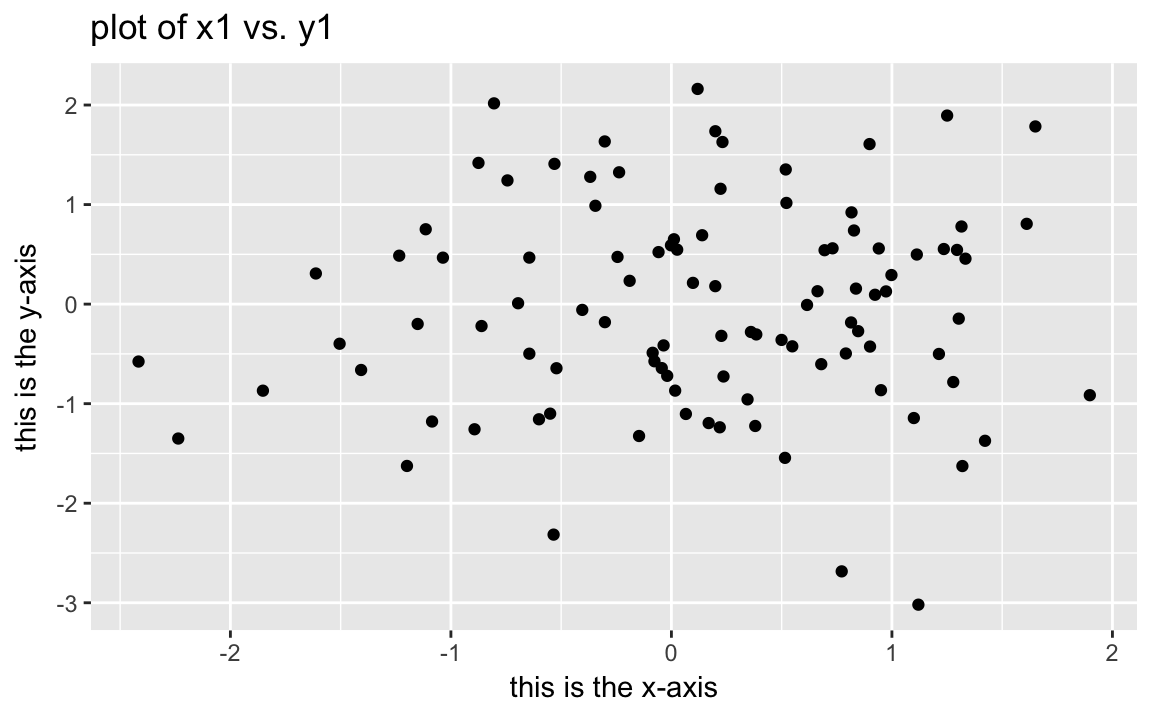
\includegraphics{tidy_islr_files/figure-latex/unnamed-chunk-1-1} \end{center}

Here is the plot.


\end{document}
